\subsection{AI Agent và Backend}

\subsubsection{Hiện thực AI Agent}

Toàn bộ hệ thống AI Agent được phát triển bằng Python. Việc lựa chọn một ngôn ngữ thống nhất giúp giảm chi phí tích hợp giữa các module, đồng thời tận dụng được hệ sinh thái thư viện mạnh cho scraping, xử lý dữ liệu và xây dựng hệ thống AI.

Kiến trúc hiện thực có thể được xem như một pipeline nhiều tầng: dữ liệu được thu thập và chuẩn hóa, sau đó được lưu trữ vào các hệ quản trị phù hợp, và cuối cùng được khai thác thông qua AI Agent và API.

\textbf{Hiện thực pipeline thu thập dữ liệu}

Pipeline thu thập dữ liệu được tổ chức thành ba bước chính: crawl URL, crawl chi tiết sản phẩm và chuẩn hóa dữ liệu. Thay vì sử dụng các request HTTP đơn thuần, hệ thống sử dụng Playwright để mô phỏng trình duyệt, cho phép xử lý các trang có nội dung động.

Ở bước crawl URL, hệ thống duyệt qua các trang danh mục và thực hiện thao tác ``xem thêm'' (load more) để thu thập toàn bộ liên kết sản phẩm. Việc sử dụng Playwright giúp đảm bảo rằng tất cả sản phẩm đều được tải, kể cả khi nội dung được render bằng JavaScript.

Ở bước crawl chi tiết, mỗi URL sản phẩm được truy cập để trích xuất thông tin bao gồm:

\begin{itemize}
\item Thông tin chung: tên, thương hiệu, dòng sản phẩm
\item Danh sách biến thể: màu sắc, giá
\item Thông số kỹ thuật
\end{itemize}

\textbf{Hiện thực tầng lưu trữ dữ liệu}

Sau khi chuẩn hóa, dữ liệu được ghi vào ba hệ quản trị theo đúng vai trò thiết kế.

Đối với PostgreSQL, dữ liệu được insert theo thứ tự product $\rightarrow$ variant $\rightarrow$ product\_spec để đảm bảo ràng buộc khóa ngoại. Các thao tác ghi được thực hiện trong transaction nhằm đảm bảo tính toàn vẹn: nếu một bước thất bại, toàn bộ dữ liệu liên quan sẽ không được lưu.

Đối với Neo4j, dữ liệu được ánh xạ thành các node và quan hệ. Việc ghi dữ liệu sử dụng câu lệnh MERGE để đảm bảo không tạo trùng node, đồng thời cho phép cập nhật khi dữ liệu đã tồn tại. Cách tiếp cận này giúp pipeline có thể chạy lại mà không gây sai lệch dữ liệu.

Đối với ChromaDB, dữ liệu văn bản (mô tả sản phẩm, FAQ, chính sách) được chia thành các đoạn nhỏ và lưu trực tiếp dưới dạng document. Hệ thống không tự tính embedding mà sử dụng cơ chế embedding tích hợp của ChromaDB để đảm bảo tính nhất quán giữa quá trình insert và truy vấn.

\textbf{Hiện thực AI Agent}

AI Agent được hiện thực dựa trên LangGraph, trong đó mỗi node trong thiết kế được ánh xạ trực tiếp thành một hàm xử lý. Trạng thái hội thoại được định nghĩa bằng lớp AgentState, cho phép chuyển đổi linh hoạt sang dạng dictionary khi tương tác với LangGraph.

Đồ thị xử lý được xây dựng thông qua Graph Builder, trong đó:

\begin{itemize}
\item Các node Parse, Resolve, Reason và Tools được khai báo rõ ràng
\item Các cạnh (edges) được định nghĩa kèm điều kiện chuyển trạng thái
\item Vòng lặp giữa Reason và Tools được hiện thực thông qua conditional edge
\end{itemize}

Luồng xử lý được biên dịch thành một graph hoàn chỉnh trước khi sử dụng. Khi nhận yêu cầu, agent chỉ cần gọi graph với trạng thái đầu vào và nhận lại trạng thái sau khi xử lý.

Các tool được triển khai như các hàm độc lập, mỗi hàm thực hiện truy vấn tới một nguồn dữ liệu cụ thể (PostgreSQL hoặc ChromaDB). Kết quả từ tool được đưa trở lại state để tiếp tục vòng suy luận.

Một điểm quan trọng trong hiện thực là việc kiểm soát lỗi. Các ngoại lệ phát sinh trong quá trình gọi tool không làm dừng hệ thống mà được đưa vào ngữ cảnh để node Reason xử lý. Điều này giúp agent có thể phản hồi linh hoạt ngay cả khi một phần hệ thống gặp lỗi.

\textbf{Hiện thực lớp API}

Lớp API được xây dựng bằng FastAPI, với endpoint trung tâm là \texttt{/api/agent/chat}. Endpoint này tiếp nhận tin nhắn người dùng và trả về phản hồi từ AI Agent.

Quản lý session được thực hiện bằng dictionary trong bộ nhớ, trong đó mỗi session chứa trạng thái hội thoại và timestamp của lần truy cập cuối. Khi có request mới, hệ thống sẽ:

\begin{itemize}
\item Dọn dẹp các session hết hạn
\item Lấy hoặc khởi tạo session
\item Cập nhật trạng thái với tin nhắn mới
\item Gọi agent graph để xử lý
\item Lưu lại trạng thái và trả về phản hồi
\end{itemize}

FastAPI lifespan được sử dụng để khởi tạo tài nguyên khi server khởi động, bao gồm:

\begin{itemize}
\item Kết nối PostgreSQL
\item Kết nối Neo4j
\item Khởi tạo ChromaDB
\item Load graph của AI Agent
\end{itemize}

Việc khởi tạo một lần tại startup giúp giảm chi phí cho mỗi request và đảm bảo hiệu năng ổn định.

Ngoài endpoint hội thoại, hệ thống còn cung cấp endpoint \texttt{/api/agent/purchase} để ghi nhận hành vi mua hàng vào Neo4j. Endpoint này kiểm tra dữ liệu đầu vào và sử dụng MERGE để đảm bảo không tạo trùng quan hệ.

\subsubsection{Hiện thực Backend}

\textbf{Kiến trúc phân lớp và điều phối luồng dữ liệu}

Tất cả các dịch vụ trong hệ thống được xây dựng trên một cấu trúc đồng nhất, áp dụng mô hình CQRS để tách biệt hoàn toàn luồng xử lý ghi dữ liệu và luồng truy vấn dữ liệu. Cấu trúc này giúp tối ưu hóa hiệu năng và tăng khả năng bảo trì hệ thống.

\begin{itemize}
    \item Nhóm Commands: Tập trung vào việc xử lý các yêu cầu thay đổi trạng thái như tạo mới, cập nhật hoặc xóa. Luồng đi từ Controller qua Service Interface đến Service thực thi và được hỗ trợ bởi các Event Handler để xử lý các sự kiện bất đồng bộ liên quan đến Kafka.
    \item Nhóm Queries: Chuyên biệt cho các tác vụ lấy dữ liệu. Luồng này được tối ưu để trả về kết quả nhanh nhất mà không cần đi qua các bước kiểm tra nghiệp vụ phức tạp của luồng ghi.
\end{itemize}

\textbf{Tổ chức đối tượng truyền tải dữ liệu DTO}

Dữ liệu trao đổi giữa client và server hoặc giữa các dịch vụ với nhau được chuẩn hóa trong thư mục dto. Các lớp này được phân chia chi tiết thành Requests và Responses cho từng loại nghiệp vụ cụ thể như auth, address, hay payment\_account. Việc tách bạch DTO cho Command và Query đảm bảo tính chặt chẽ của dữ liệu đầu vào và đầu ra, tránh việc phơi bày các thực thể cơ sở dữ liệu trực tiếp ra bên ngoài.

\textbf{Tầng truy xuất dữ liệu Repository}

Tương ứng với mô hình CQRS, tầng Repository được chia làm hai loại:

\begin{itemize}
    \item jpa\_repositories: Sử dụng Spring Data JPA để thực hiện các thao tác lưu trữ và cập nhật vào cơ sở dữ liệu.
    \item read\_only\_repositories: Được cấu hình tối ưu chỉ để đọc dữ liệu, giúp giảm tải cho hệ thống và tăng tốc độ phản hồi cho các yêu cầu truy vấn.
\end{itemize}

\textbf{Các thành phần hỗ trợ hệ thống}

\begin{itemize}
    \item Mapper và Factory: Tầng mapper chịu trách nhiệm chuyển đổi dữ liệu giữa Model và DTO một cách tự động. Tầng factory được sử dụng để khởi tạo các đối tượng phức tạp, đảm bảo tính đóng gói của mã nguồn.
    \item Email Handler và Util: Các tác vụ bổ trợ như gửi email thông báo được tách thành module riêng để không gây nghẽn luồng xử lý chính. Các hàm tiện ích dùng chung được tập trung tại util để tái sử dụng trên toàn dịch vụ.
    \item Config: Chứa toàn bộ các cấu hình hệ thống bao gồm cấu hình bảo mật, cấu hình Kafka và cấu hình kết nối cơ sở dữ liệu.
\end{itemize}

\textbf{Tổ chức module common như một thư viện nội bộ}

Module common được xây dựng như một thư viện dùng chung cho toàn bộ các microservices. Module này chứa các thành phần cốt lõi như cấu hình JWT Security, Global Exception Handling và các DTO dùng chung cho việc giao tiếp qua Kafka. Module này được đóng gói thành một dependency và được thêm vào file cấu hình Maven của từng dịch vụ, giúp đảm bảo tính đồng nhất về xử lý lỗi và cấu trúc dữ liệu trên toàn hệ thống.

\subsubsection{Triển khai AI Agent và Backend}

Toàn bộ hệ thống được triển khai trên nền tảng điện toán đám mây Microsoft Azure, sử dụng máy ảo để vận hành đồng thời các dịch vụ Backend, AI Agent và hạ tầng hỗ trợ.

\textbf{Thông số hạ tầng máy ảo}

Hệ thống được vận hành trên một máy ảo với cấu hình cụ thể như sau:

\begin{itemize}
    \item Cấu hình: Standard B2als v2 (2 vCPUs, 4 GiB memory).
    \item Hệ điều hành: Linux (Ubuntu Server).
    \item Vị trí: Southeast Asia (Zone 1).
    \item Địa chỉ IP Public: 57.155.x.xxx.
\end{itemize}

\begin{figure}[H]
    \centering
    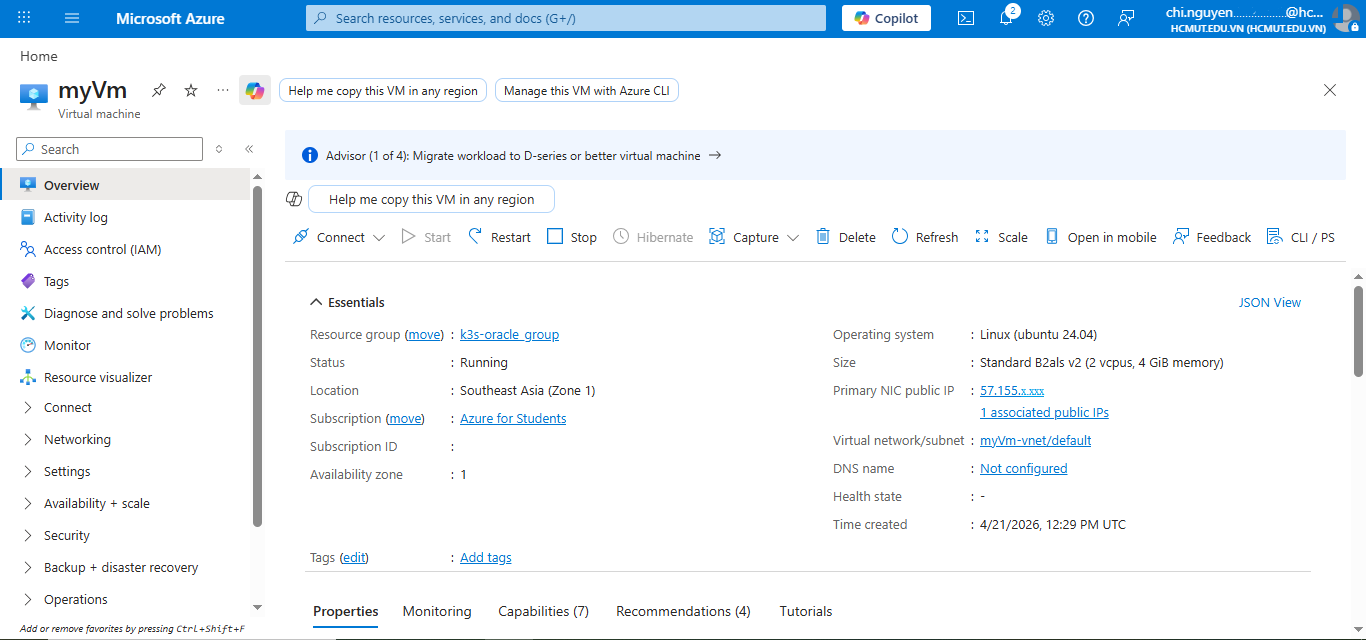
\includegraphics[width=0.9\textwidth]{images/chap7/backend/azure_machine.PNG}
    \vspace{0.7 cm}
    \caption{Giao diện quản lý Virtual Machine (myVm) trên Microsoft Azure Portal}
    \label{fig:azure_vm}
\end{figure}

Kiến trúc triển khai và điều phối hệ thống

Toàn bộ hệ thống được triển khai theo mô hình tập trung trên một máy ảo Azure, trong đó các thành phần Backend, AI Agent và hạ tầng hỗ trợ được đóng gói dưới dạng container Docker nhằm đảm bảo tính nhất quán trong môi trường thực thi và thuận tiện cho quá trình quản lý.

Hệ thống sử dụng Docker Compose để điều phối container, thiết lập mạng nội bộ và quản lý kết nối giữa các service. Các thành phần chính bao gồm:

\begin{itemize}
    \item API Gateway là thành phần duy nhất được mở cổng ra Internet thông qua Azure Network Security Group, chịu trách nhiệm tiếp nhận request từ client và điều phối đến các service bên trong hệ thống.
    \item Các dịch vụ nghiệp vụ được triển khai dưới dạng container Java Spring Boot và chỉ hoạt động trong mạng Docker nội bộ nhằm hạn chế truy cập trực tiếp từ bên ngoài.
    \item AI agent được triển khai như một container Python độc lập, chịu trách nhiệm xử lý các truy vấn thông minh và tích hợp mô hình ngôn ngữ lớn. Vector database được lưu trữ cục bộ và gắn trực tiếp với AI agent để phục vụ truy vấn ngữ nghĩa.
    \item Cơ sở dữ liệu quan hệ PostgreSQL được triển khai trên nền tảng Supabase dưới dạng dịch vụ quản lý toàn phần. Các service kết nối đến cơ sở dữ liệu thông qua connection string được cấu hình bằng biến môi trường.
    \item Hệ thống message queue Kafka được triển khai trực tiếp trên máy ảo Azure thông qua Docker Compose nhằm phục vụ cơ chế giao tiếp bất đồng bộ giữa các microservices.
    \item Docker Compose thiết lập mạng bridge nội bộ cho phép các container giao tiếp với nhau thông qua service name mà không cần public endpoint nội bộ ra Internet.
\end{itemize}

Thiết kế kiến trúc này giúp giảm tải công tác quản trị cơ sở dữ liệu quan hệ nhờ sử dụng dịch vụ managed database, đồng thời vẫn duy trì khả năng kiểm soát hạ tầng xử lý message queue và các service nghiệp vụ ngay trên môi trường triển khai thực tế.

\textbf{Quy trình đóng gói và triển khai Docker Image}

Ở giai đoạn đầu, các service nghiệp vụ Java được build thành file \texttt{.jar} và chuyển thủ công lên máy ảo để triển khai. Tuy nhiên, sau khi tích hợp thêm AI Agent sử dụng Python, hệ thống được chuyển sang phương pháp đóng gói toàn bộ service thành Docker Image để đồng nhất môi trường thực thi.

Quy trình triển khai hiện tại được thực hiện như sau:

\begin{itemize}
    \item Mỗi service được định nghĩa bằng một Dockerfile riêng biệt phù hợp với runtime tương ứng.
    
    \item Các service nghiệp vụ Java được đóng gói thành Docker Image sử dụng môi trường JRE nhẹ nhằm giảm dung lượng image và tối ưu tài nguyên hệ thống.
    
    \item AI Agent được đóng gói cùng toàn bộ thư viện Python cần thiết phục vụ xử lý AI.
    
    \item Sau khi hoàn tất kiểm thử tại môi trường phát triển, Docker Image được build cục bộ và push lên Docker Registry.
    
    \item Tại máy ảo Azure, hệ thống sử dụng \texttt{docker compose pull} và \texttt{docker compose up -d} để cập nhật và khởi động các service.
\end{itemize}

Cách triển khai này giúp đơn giản hóa quá trình cập nhật phiên bản, giảm sai lệch môi trường giữa development và production, đồng thời hỗ trợ triển khai đồng nhất cho cả các service nghiệp vụ và service AI.

